\section{Case Study: Four Time-Series Foundation Models}
\label{sec:casestudy}

\subsection{Setup}
\label{sec:setup}

We analyze TimesFM~2.5, Chronos-2, Sundial and Chronos-Bolt (Table~\ref{tab:models}) with the preset
\repo{tsfm_lens/configs/concept_atlas_v2.yaml}. The dev corpus has 965 series in five generator families
(\texttt{parametric}, \texttt{random\_parametric}, \texttt{mixture}, \texttt{block\_bootstrap},
\texttt{sequential\_par}); the real-derived families draw on Monash weather, ETT \citep{zhou2021informer}
and the Chronos electricity and traffic collections. Contexts are 512 steps, the horizon is 64 and the
alignment window is 32. SAEs are trained on 29 target layers (TimesFM: 10, at stride 2; Chronos-2: 7;
Sundial: 9; Chronos-Bolt: 3), with three replicate seeds each for stability, and $n_{\text{boot}}=2000$
throughout. The private split is 800 sealed series (epoch 0 of the v2 benchmark), opened once. The whole
run took 6.43 hours on a single NVIDIA RTX A5000 (24~GB), of which SAE training took 2.39 hours and the
concept stage 3.72 hours (Appendix~\ref{app:repro}). All artifacts are in
\repodir{examples/concept_atlas_v2/run}; results that come from other runs recorded in the ledger are
marked with their \repo{FINDINGS.md} identifier.

Before turning to the research questions, Table~\ref{tab:character} summarizes the models' behavior,
which later sections use as context. Chronos-2 is the most accurate on the dev corpus and on held-out
data. Sundial covers only 37\% of outcomes with its nominal 80\% interval. TimesFM and Sundial propagate
an injected NaN to the forecast without raising, while the Chronos models handle it. Behind the Sundial
row is a bug found during this work: the first Sundial adapter bypassed the checkpoint's input
normalization, and the \texttt{frontend} stage's scale-equivariance residual (38.43 context standard
deviations, against $\le 0.009$ for the other models) was at first read as a property of the model
(\fid{PM-15}; Section~\ref{sec:controls}). After the fix the residual is 0.033.

\begin{table}[t]
\centering
\footnotesize
\setlength{\tabcolsep}{4pt}
\begin{tabular}{@{}lccccc@{}}
\toprule
Model & median MASE & 80\% coverage & scale resid.\ ($\times$0.001) & NaN input & latency \\
\midrule
\textcolor{ctwo}{Chronos-2}    & \textbf{1.1251} & 0.772 & 0.0093 & handled & 21 ms \\
\textcolor{tfm}{TimesFM}       & 1.1829 & \textbf{0.795} & $2.0\times10^{-6}$ & propagates & 38 ms \\
\textcolor{sun}{Sundial}       & 1.3335 & 0.369 & 0.0332 & propagates & 7 ms \\
\textcolor{bolt}{Chronos-Bolt} & 1.4913 & 0.749 & 0.0087 & handled & 14 ms \\
\midrule
naive / seasonal naive & 2.6829 / 2.0280 & & & & \\
\bottomrule
\end{tabular}
\caption{Behavioral character on the v2 dev corpus (965 series). Scale residual: error of
$f(c\,x)/c$ against $f(x)$ in context standard deviations. Held-out, Chronos-2 is more accurate
than TimesFM overall (paired $\Delta$MASE $-0.148$ [$-0.211$, $-0.088$], $p=0.0005$, $n=800$).
Source: \texttt{l0/summary.json}, \texttt{l0/calibration.json}, \texttt{frontend/frontend.json},
\texttt{confirm/confirmation.json}.}
\label{tab:character}
\end{table}

\subsection{RQ1: What forecast-relevant concepts do TSFMs learn?}
\label{sec:rq1}

\paragraph{Causal features exist, and the battery discriminates.} Across the 29 targets, 293 SAE features
clear the row-matched random-direction null on at least one of the nine forecast channels. Twenty-eight
targets passed both reach controls (for example, TimesFM \texttt{stacked\_xf.10}: self-patch exactly 0.0,
cross-patch relative reach 0.146). The twenty-ninth, Chronos-2's final block, was withheld: patching another
layer into it moved the forecast by exactly 0, because Chronos-2's head reads forecast placeholder tokens that
a patch of the context positions never reaches (\fid{DE-03}). Without the reach probe this target would have
reported a full table of zero effects (\texttt{sae/concept\_stage.json}). The battery is selective rather than
permissive: on the reference four-model run, (feature, channel) cells clear the null at 2.49 to 6.61 times
the rate expected by chance, and features nominated at random clear at about half the rate of features
nominated by activation rules (\fid{MP-07}).

\paragraph{The concepts are about level and shape.} Figure~\ref{fig:families} shows the nine effect families
that tile the causal features. The three largest (148 of 288 assigned features) act on forecast level and
volatility: \emph{Level lowerers} (80), \emph{Level raisers \& Accuracy improvers} (61) and
\emph{Volatility dampeners} (48). Families whose defining channel is trend or seasonality are smaller:
\emph{Trend boosters \& Accuracy improvers} (23), \emph{Trend dampeners} (18), \emph{Seasonality amplifiers}
(17) and \emph{Trend boosters \& Volatility amplifiers} (12). Nearly every family also moves the near- and
far-horizon shape distances. Level is not the whole story, however: on the reference run the median share
of a causal feature's effect that is a pure level shift is 0.535, and most causal features still clear a
null after the level shift is removed from both the feature and the null (\fid{CA-07}).

\begin{figure}[t]
\centering
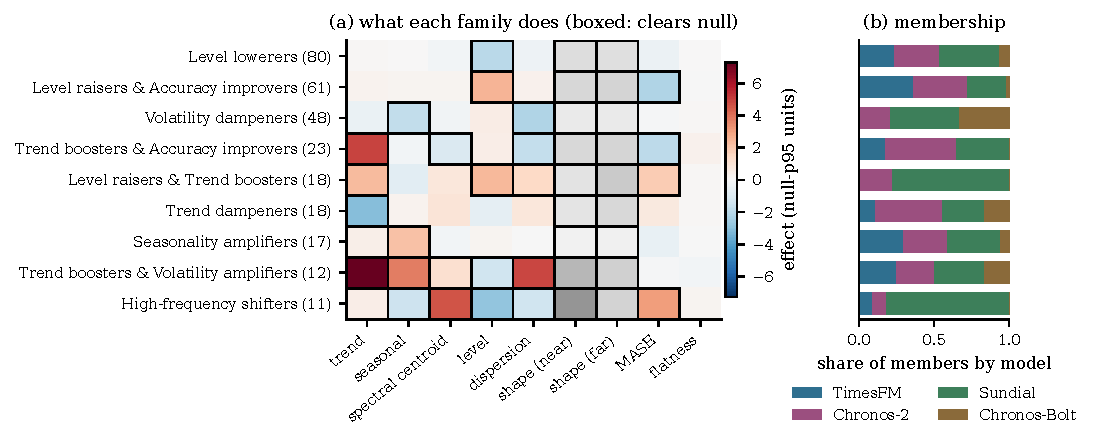
\includegraphics[width=\textwidth]{figures/families.pdf}
\caption{The nine causal-effect families of the example run, ordered by size. (a) Family centroid in
null units: what removing a member does, negated to state what the feature \emph{does}; red raises the
channel and blue lowers it. Boxed cells clear the null in the family description. The near- and
far-horizon shape channels are distances, drawn unsigned in gray. (b) Membership by model: families are
populated unevenly by model. Source: \texttt{sae/concept\_families.json}; regenerated by
\texttt{paper/figures/make\_figures.py}.}
\label{fig:families}
\end{figure}

\paragraph{The concepts are graded, not discrete.} Three observations indicate that ``concept'' should be
read as a region of a continuous effect space rather than as a discrete unit. First, clustering within a
layer rarely finds modules: 24 of 29 targets are non-modular, yielding only 9 per-target concepts. Second,
the strict atlas assigns only 86 of 293 features (29\%) to its 27 concepts. Third, the nine readable
families cover 288 of 293 features (98\%) but do \emph{not} beat a column-shuffle null (permutation
$p=1.0$ for the number of families and $p=0.985$ for coverage). A similar picture holds on the reference run,
where silhouette is 0.31--0.35 for every family count from 3 to 16 (\fid{CA-10}), and the 9-channel
ablation fingerprints have a participation-ratio dimension of only 2.09 (\fid{MN-07}). The families are
therefore a useful vocabulary for reading the report, and the paper uses them in that sense only.

\paragraph{Concepts named after ground truth are rare, and naming them requires a null.} Because the
benchmark records every generative component, \tool{} can ask whether a feature tracks a known field.
Some do: after dead-feature revival, 154 of 10{,}240 TimesFM features and 115 of 6{,}144 Chronos-T5-Base
features match a ground-truth field beyond a permutation null, the best being a Chronos feature tracking
intermittency at $\rho=0.881$ (\fid{MP-06}). But raw correlations do not separate trained from untrained
weights (an untrained twin scores 0.565 against 0.567), so only the margin over the null is evidence. Two
tempting stronger claims failed their tests. Validating concepts by moving a generator knob and watching the
concept respond was a confirmed negative, twice: 0 of 98 and then 0 of 151 knob--concept pairs survived
correction, because a knob moves any active feature about as much as the targeted one (\fid{MN-17}).
And a vivid TimesFM ``random walk'' concept (19 of 20 top series from the random-walk archetype; ablation
worsens MASE by 4.04 times the null) failed the seed-stability test and is not promoted (\fid{PM-11}).

\paragraph{Answer to RQ1.} TSFMs contain sparse, causally effective directions, and what they control is
mainly the level, volatility and shape of the forecast, with trend and seasonality handled by smaller
groups. These directions form a continuum with a few dominant axes rather than a set of discrete, named
concepts, and they are not specific to the generative factors a practitioner would name.

\subsection{RQ2: Are concepts shared across architectures?}
\label{sec:rq2}

\paragraph{Geometry is shared above chance, but ``similarity'' has no single meaning.} Peak linear CKA
between TimesFM and each other model is 0.38--0.43, against a shuffled-series null of 0.037, and the
TimesFM/Chronos-2 peak replicates on private data (dev 0.4262; private 0.4253 [0.4162, 0.4423]). The same
above-null band holds across five unrelated architectures, including Timer through the zero-code adapter
(0.449, null 0.063) and Lag-Llama (\fid{SH-01}). The three models with 16-step tokens are far more similar to
each other (0.909--0.928). Figure~\ref{fig:similarity} shows, however, that seven pair-similarity metrics
rank the six pairs inconsistently (Kendall's $W=0.28$, permutation $p=0.07$). TimesFM/Chronos-2 is the most
similar pair by error agreement (Spearman 0.947 across series), and only fourth by CKA and stitching gain.
\tool{} therefore never pools the metrics into one similarity score. Two further controls limit what
similarity means. An untrained pair of the same architecture is more CKA-similar (0.878) than a genuinely
related trained pair (0.734; difference $p=0.0005$), so representational similarity cannot detect model
lineage (\fid{MN-01}). And an attractive unit-level correspondence measure rose, rather than fell, when both
bases were randomly rotated (0.148 to 0.331), because TSFM layers are so low-rank (participation ratio as
low as 1.54) that every direction correlates with the same few components (\fid{SH-19}).

\begin{figure}[t]
\centering
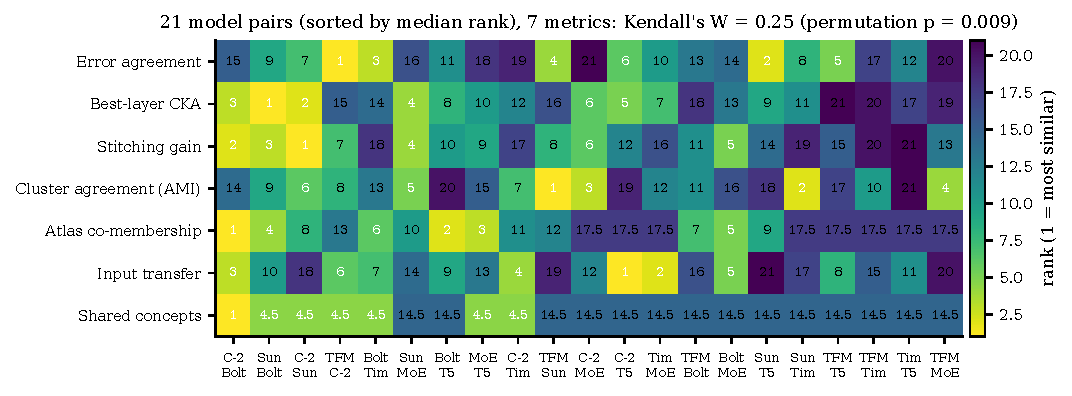
\includegraphics[width=0.66\textwidth]{figures/similarity.pdf}
\caption{Rank of each model pair (columns) under seven similarity metrics (rows); 1 is most similar.
Behavioral, geometric, translational, clustering and concept-level metrics disagree about which models are
alike. Source: \texttt{report/model\_similarity.json}.}
\label{fig:similarity}
\end{figure}

\paragraph{Models agree on which inputs a concept groups.} Concept transfer asks whether another model has a
feature that picks out a concept's top series. At atlas scale, 1{,}223 of 1{,}581 transfer tests (77\%) are
reciprocal after Benjamini--Hochberg correction. Twenty claims were registered from dev results alone and
tested once on the 800 private series: all 20 were confirmed under Holm correction (maximum adjusted
$p=0.0100$; private AUC 0.971--0.995 against null 95th percentiles of 0.57--0.77; Figure~\ref{fig:heldout}b).
This result has now replicated on three independent private draws: 19 of 20 in search mode on v1 epoch~1,
20 of 20 with frozen feature pairs on epoch~2, and 20 of 20 on v2 (\fid{SH-18}). Two caveats bound it. It is
an \emph{input-level} claim (the same series are grouped by both models), not a causal one. And the 20 v2
claims come from only two concepts, with only 6 of 20 private best features identical to the dev ones, so
the replicated statement is that the destination layer has \emph{some} feature that selects the same
series.

\paragraph{Models rarely agree on what a concept does.} Figure~\ref{fig:funnel} follows the candidates up
the evidence ladder. Of the 27 atlas concepts, 16 contain causal members from at least two models, but only
two are \emph{shared} (same effect and same inputs) and one is partially shared. The dominant class is
\emph{convergent} (13 concepts): features in different models have the same causal effect on
\emph{different} series. Eleven concepts belong to a single model. Restricted to the 22 seed-stable
concepts, the counts are 9 convergent, 10 single-model, 2 shared and 1 partially shared. No concept has
causal members in all four models; one spans three. The direct test agrees. Of the 1{,}223 reciprocal
transfers, 420 are scorable (both sides clear their own null on the shared series), and among those only 11
(2.6\%) show the same causal effect, 81 agree on level or shape alone, 264 show no specific agreement, and
64 (15.2\%) act measurably differently. The family memberships in Figure~\ref{fig:families}b tell the same
story: the families are segregated by model.

\begin{figure}[t]
\centering
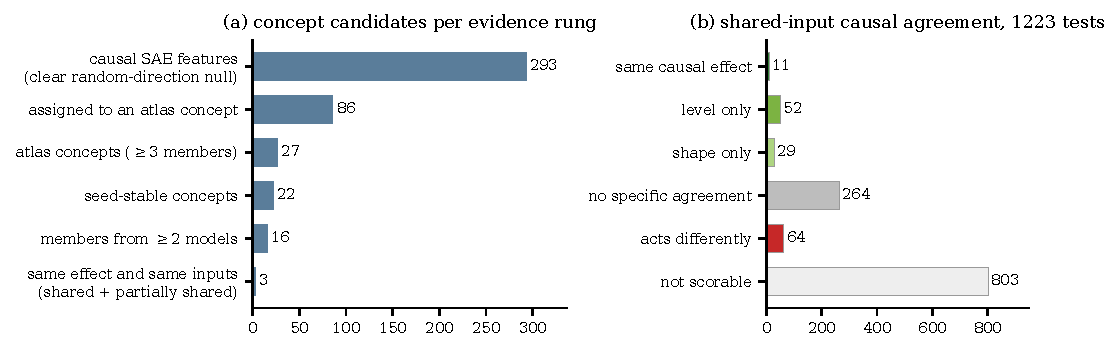
\includegraphics[width=\textwidth]{figures/funnel.pdf}
\caption{(a) Number of concept candidates at each rung. The first three bars count features and concepts
in sequence; the last three are separate properties of the 27 atlas concepts. (b) Verdicts of the
shared-input causal agreement test over all 1{,}223 reciprocal-FDR transfers; ``acts differently''
requires a lower-tail result against matched floors. Source: \texttt{sae/concept\_stage.json}.}
\label{fig:funnel}
\end{figure}

\paragraph{Answer to RQ2.} Different TSFMs \emph{detect} the same things: a concept learned by one model
selects series that another model's dictionary also selects, reliably enough to replicate on sealed data.
They mostly do not \emph{use} them the same way: effects shared on the same inputs are rare, the typical
multi-model concept is convergent, and no concept is common to all four models. Whole-layer similarity
metrics cannot reveal this distinction, and they disagree with each other.

\subsection{RQ3: Do concepts causally affect the forecast, and how much?}
\label{sec:rq3}

The ablation battery establishes causality at the level of single features: every concept in
Section~\ref{sec:rq1} is built from features that move the forecast more than a matched random removal does,
on the series they fire on, with reach verified. How much of the forecast these features account for is
a separate question, and the answer is: individually, little. On the reference run, the median effect of
removing one feature is 0.0395 context standard deviations, while replacing the layer by its SAE
reconstruction already moves the forecast by 0.139, 3.5 times more (\fid{MN-15}). Of 565 features that the
report would otherwise display as ``interesting'' because they activate strongly, 364 (64.4\%) clear no
causal channel at all (\fid{MN-14}); \tool{} collapses them rather than rendering them as findings. Causality
also depends on the dictionary: reviving dead atoms, which improves fidelity, reduced ground-truth
alignment at every TimesFM depth tested (from $-0.030$ to $-0.132$) while the causal signal fell much less,
and rose in one Chronos-2 layer (2.27 to 4.06 times chance; \fid{MN-21}).

Head-level analyses show the same gap between what looks important and what is. The correlation between
the attention mass a head places on seasonal lags and the seasonal power lost when that head is ablated is
$\rho=0.026$ in TimesFM and $\rho=-0.118$ in Chronos-T5-Base (\fid{CA-04}), in line with the
language-model finding that attention weights are not explanations \citep{jain2019attention}. A minimal
circuit restoring seasonality under \texttt{deseasonalize} consists of one head in TimesFM ($p=0.04$) but
five non-additive heads in Chronos-T5-Base ($p=0.008$; \fid{CA-03}).

\paragraph{Answer to RQ3.} Yes, causally, in the controlled sense: individual features and heads change the
forecast in specific, null-beating ways. But no single feature carries much of the forecast, most
prominent features carry nothing, and attention patterns are unreliable guides to which components matter.
Causal claims about TSFM concepts are claims about small, distributed contributions.

\subsection{RQ4: Where in depth, and how comparable is depth?}
\label{sec:rq4}

The corruption fingerprints locate where each model's activations react to a structural change of the
input, and their cross-model agreement is one of the most robust results in the ledger. For the registered
pair TimesFM/Chronos-2, all nine per-corruption agreements replicate on private data (overall $\rho=0.510$
[0.489, 0.527]; Figure~\ref{fig:heldout}a): the two models react at \emph{matching} depths to detrending,
deseasonalizing, frequency shifts and dropout, and at \emph{opposite} depths to noise ($\rho=-0.742$),
spikes ($-0.780$), warps ($-0.658$) and smoothing ($-0.466$). Whole-layer restoration can hide depth
structure: in TimesFM it is flat across depth, yet per window it concentrates in the window just before the
horizon and intensifies with depth (for \texttt{noise}, from 0.068 at layer 0 to 0.412 at layer 16;
\fid{DE-01}).

Comparing depth \emph{locations} across architectures, however, needs two qualifications that \tool{}
computes and renders for every run. The captured share of a forecast's computation ranges from 22\%
(Sundial, whose sampled head runs outside the captured pass) to 98\% (Chronos-2), and for Chronos-T5-Base,
where 100\% of encoder blocks are captured, it is only 14\% (\fid{DE-05}). And on a whole-stack depth axis,
Chronos-T5's last encoder block sits at 0.478, so the comparable depth range with TimesFM is only half the
axis (\fid{DE-04}). Which layers are ``interesting'' also depends on the selector: a specification curve over
three selectors found no selected layer robust for any model (\fid{DE-08}). Across a five-size Chronos-T5
scaling ladder (8M to 709M parameters), only family decodability increased monotonically with size
(\fid{DE-07}).

\paragraph{Answer to RQ4.} Depth-resolved reaction profiles are reproducible and reveal which structural
properties two models process at the same relative depth. Absolute depth locations are comparable across
architectures only after accounting for captured compute and for the depth convention, which \tool{} reports
alongside every depth claim.

\subsection{What replicated on held-out data}
\label{sec:heldout}

\begin{figure}[t]
\centering
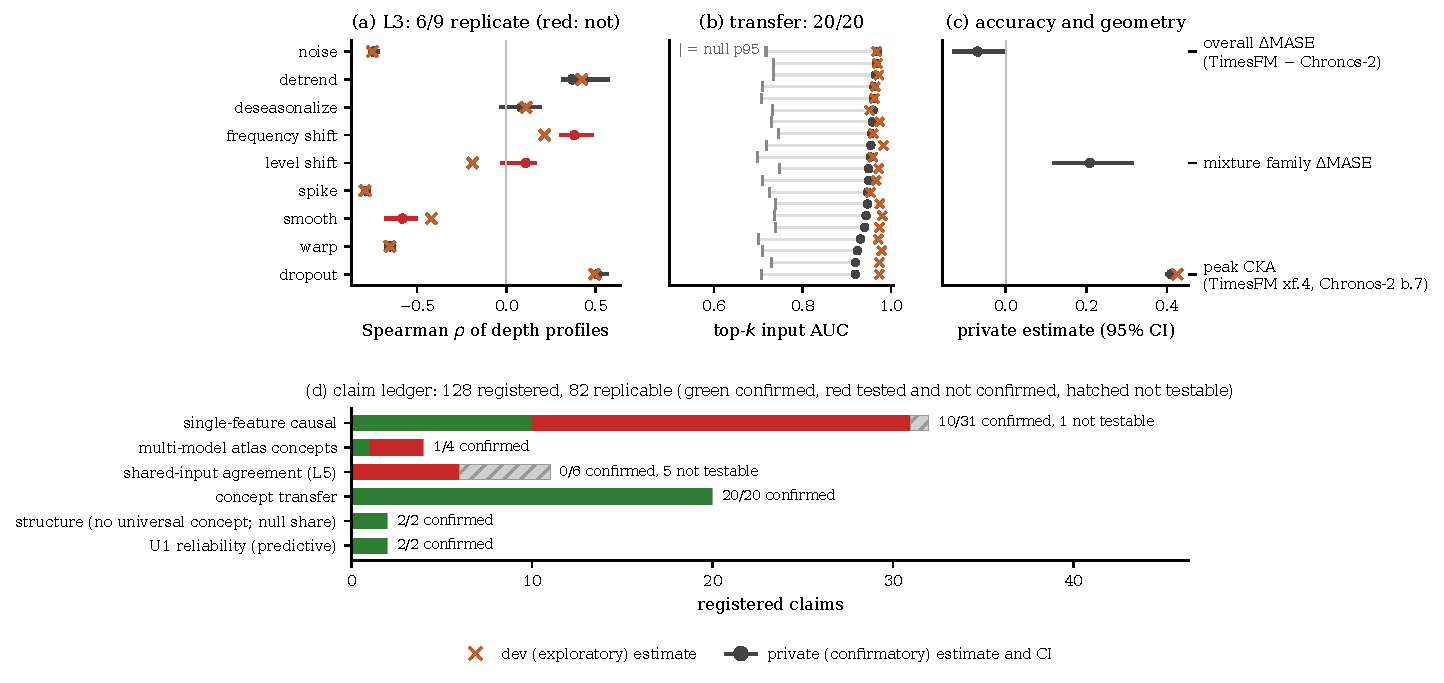
\includegraphics[width=\textwidth]{figures/heldout.pdf}
\caption{Every claim re-tested on the 800 sealed private series. (a) Per-corruption depth-profile agreement
between TimesFM and Chronos-2; (b) the 20 registered concept-transfer claims, with each claim's private null
95th percentile; (c) accuracy and peak CKA. Crosses: dev estimates; dots and bars: private estimates with
95\% series-bootstrap intervals. Source: \texttt{confirm/confirmation.json}.}
\label{fig:heldout}
\end{figure}

The \texttt{register} stage recorded 47 hypotheses, 31 of which the \texttt{confirm} stage can currently
re-test (L2 stitching, archetype-level accuracy and clustering claims are registered but not yet
replicable, and the report lists them as such). Every re-tested claim held (Figure~\ref{fig:heldout}): the
registered accuracy claim (Chronos-2 more accurate on \texttt{mixture}, $\Delta$MASE 0.307 [0.209, 0.413],
$p_{\text{Holm}}=0.0005$, $n=240$, where the minimum detectable effect had been 0.155), the peak-CKA pair, all
nine perturbation agreements and all 20 concept-transfer claims. Table~\ref{tab:results} collects the headline
results with their evidence class and status. What did \emph{not} undergo held-out testing matters equally:
the causal concept results of Sections~\ref{sec:rq1}--\ref{sec:rq3}, including the sharing classes and the
shared-input agreement counts, are exploratory. They were, however, reproduced on a second corpus: on the
v1 reference run, 0 of 19 atlas concepts span all four models, convergent is again the most common class,
and 12 of 89 scorable shared-input tests act differently (\fid{SH-16}, \fid{CA-06}).

\begin{table}[t]
\centering
\footnotesize
\setlength{\tabcolsep}{3pt}
\begin{tabularx}{\textwidth}{@{}l>{\raggedright}Xllll@{}}
\toprule
RQ & Result (example run unless an ID is given) & Evidence class & Status & ID \\
\midrule
1 & 293 causal features; 9 families, largest act on level/volatility & causal within-model & exploratory, 2 corpora & CA-10 \\
1 & Families cover 98\% but do not beat a shuffle null ($p=1.0$) & descriptive & exploratory, 2 corpora & CA-10 \\
1 & Knob-specific concept mediation: 0/98, then 0/151 & correlational & confirmed negative & MN-17 \\
2 & Peak CKA 0.425 vs null 0.037 & geometric & held-out confirmed & SH-01 \\
2 & 7 similarity metrics disagree ($W=0.28$) & mixed & exploratory & SH-05/06 \\
2 & Untrained pair more similar than related trained pair & geometric & confirmed negative & MN-01 \\
2 & Concept transfer on inputs: 20/20 & correlational & held-out confirmed (3 draws) & SH-18 \\
2 & No 4-model concept; convergent is the modal class & causal, compared & exploratory, 2 corpora & SH-16 \\
2 & Same effect on same inputs: 11/420 scorable & causal on shared inputs & exploratory, 2 corpora & CA-06 \\
3 & Feature effect 3.5$\times$ below SAE reconstruction cost & causal within-model & exploratory & MN-15 \\
3 & 64\% of prominent features causally null & causal within-model & exploratory & MN-14 \\
3 & Attention mass uncorrelated with head causality & causal vs.\ descriptive & exploratory & CA-04 \\
4 & Depth-profile agreement, 9/9 corruptions & causal within-model & held-out confirmed & CA-01 \\
4 & Captured compute 14\%--98\% qualifies depth claims & descriptive & confirmed & DE-05 \\
\midrule
L0 & Chronos-2 more accurate than TimesFM ($-0.148$) & behavioral & held-out confirmed & PM-05 \\
\bottomrule
\end{tabularx}
\caption{Headline results with evidence class and confirmation status. Each ID links to its entry in
\repo{FINDINGS.md}, which gives exact numbers, the reproduction command and the artifact path.}
\label{tab:results}
\end{table}
